\part{Notes}

Space debris
Radiation - hardened hardware
Explain van Allen Belts? Picture in earlier sections as per Falke and Letterio theses
\begin{figure}
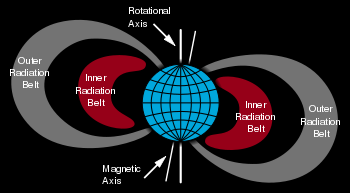
\includegraphics[width=\textwidth]{Images/350px-Van_Allen_radiation_belt_svg.png}
\caption{The van Allen Belts conceptual image}\label{fig:vabs}
\end{figure}
outer radiation belt extends from an altitude of about three to ten Earth radii, and is characterised by a relatively high density of high energy (0.1-10~MeV) electrons trapped within Earth's magnetosphere. The density varies wildly based on geomagnetic storms and variations in solar wind.
much more worrying is the inner belt which extends from an altitude of 100~km (the edge of space) to about 10,000~km, and consists of high concentrations of energetic protons (some over 400~MeV, which can penetrate 143~mm of lead) thought to be caused by cosmic ray collisions with nuclei of the upper atmosphere.
\begin{figure}
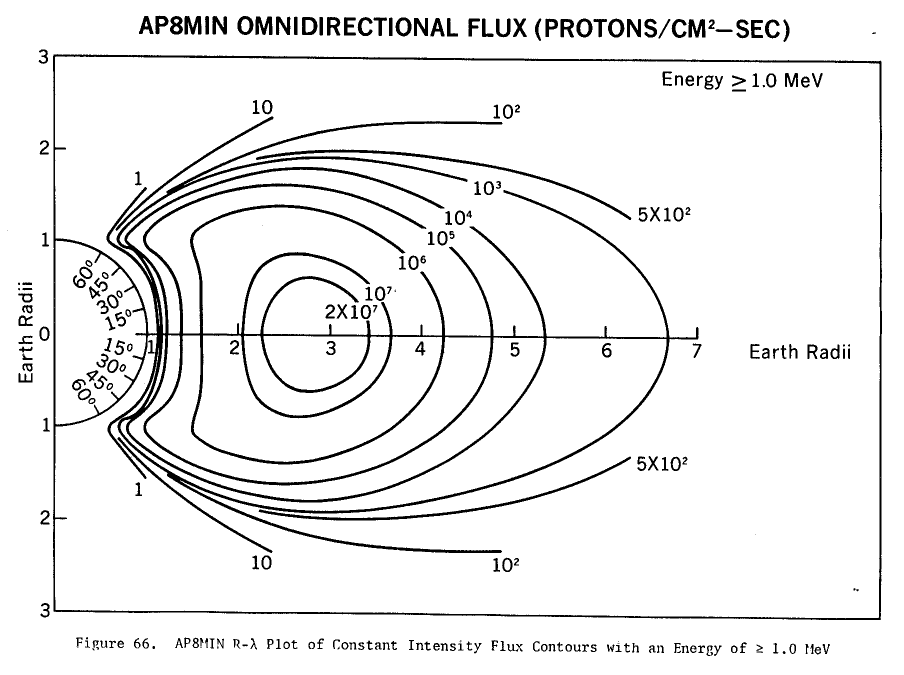
\includegraphics[width=\textwidth]{Images/Ap8-omni-1_000MeV.png}
\caption{The van Allen Belts proton flux distribution \parencite{Sawyer1976}.}\label{fig:vabs}
\end{figure}
reaction wheels for attitude control; at the moment no external thrusters for attitude control. It has been suggested to use the PPTs for reaction wheel desaturation, although they can only remove pitch and yaw, not roll.

% ------------------------------------------------------------------------------------------------

Copy new sections from IAC paper 2010 \textcite{Shimmin2010}

\begin{enumerate}
\item Rewrite 1.1 outline
\item 2 what i have achieved (gap)
\item 2.5 Scope
\item 3.3 Optimisation methods and pictures
\item 4 corel draw for coordinate diagrams
\end{enumerate}

give ground access times from STK

\enquote{While the lunar orbit in DE 421 is close to that in DE 418, it is a major improvement over the widely distributed DE 405 (Standish 1998). For DE 405 the lunar orbit was not fit in a way consistent with the other planets}\cite{DE421}.

Ephemeris Time, used by the \textcite{NAIF2010}. Number of seconds since J2000 epoch.


ITRF - international terrestrial reference frame \url{http://itrf.ensg.ign.fr/} for oblateness

Lunar reference frames \url{http://naif.jpl.nasa.gov/naif/lunar_kernels.txt} \textcite{LCF}.

third body forces from Jupiter barycenter

The geographic parameters of satellite radius $r$, longitude $\lambda$ and latitude $\phi$ are calculated by converting the ECI frame to a body-fixed frame. The conversion is provided by the International Earth Rotation Service \parencite{Petit2010}.

Define J2000 frame and epoch

The IERS Celestial Reference Frame (ICRF) is offset from the J2000 reference frame (equivalent to EME 2000) by a small rotation:  the J2000 pole offset magnitude is about 18 milliarcseconds (mas) and the equinox offset magnitude is approximately 78 milliarcseconds (see [3]). \url{http://naif.jpl.nasa.gov/pub/naif/GRAIL/kernels/fk/moon_080317.tf}

The ITRF93 high accuracy Earth rotation model takes into account:
\begin{itemize}
\item Precession: 1976 IAU model due to Lieske.
\item  Nutation: 1980 IAU model, with IERS corrections due to Herring et al.
\item  True sidereal time using accurate values of TAI-UT1
\item  Polar motion
\end{itemize}



backwards propagation allows optimisation of mass - once final dry mass is known, can propagate backwards to determine how much wet mass is required.


\cite{Yam2011} attempts global search using basin hopping and simulated annealing, each hybridized with a local search algorithm. Has to approximate the low thrust maneouvre as a series of impulsive maneouvers.
cartesian state
theoretical nuclear electric mission to Jupiter, 2.26~N, 6000~s, 20000~kg with gravitational swing-bys.
another one to Mercury, 1300~kg, 0.34~N and 3200~s.


homotopy/embedding/continuation methods: optimise a simplified case (two body problem), then use that solution as the initial guess for a more sophisticated case, etc.


direct transcription
\begin{subequations}
\begin{gather}
n \approx (n_y + n_u)MN \\
n_y = 8 \\
n_u = 4 \\
M = 4 optimisable phases \\
N = 80,000 grid points per phase \\
=2.56e6 \\
\end{gather}
\end{subequations}
\cite{Betts1998}

SOCS implements a sparse SQP method based on a Schur-complement algorithm suggested by Gill et al. (Stanford technical papers)

Jacobian and Hessian matrices are computed efficiently using sparse finite differencing as proposed by \cite{Coleman1983} SIAM journal of numerical analysis and \cite{Curtis1974} Journal of the Institute of Mathematics and Applications

\section{SOCS output}
No DOF : number of parameters minus active constraints. Approx 50,000 for Cruise phase
Cond KKT system: condition number of Hessian matrix of Lagrangian, from Newton's method: $A\vec{x}=\vec{b}$ where $A$ is the Hessian, $\vec{x}$ is the system and $\vec{b}$ represents the perturbations. A high condition number means the system is highly sensitive to small changes in the perturbation vector. Approx 1e11

SOCS uses BFGS (Broyden-Fletcher-Goldfarb-Schanno) quasi-Netwon method to approximate Hessian .

Cruise with NASA libraries: 200000000 doubles and 80000000 words
1e-4 opt tolerance, 1e-5 constraint tolerance, 2e-5 ODE tolerance



tangential thrusting is optimal to raise periapsis
eclipse should be avoided, especially at apoapsis
thrust in velocity vector to increase semimajor axis 
\textcite{Racca9}


\cite{Cabrera2011} for info about russian PPTs running at 10+~Hz